\documentclass[a4paper, 11pt]{article}
\usepackage{comment} % enables the use of multi-line comments (\ifx \fi) 
\usepackage{fullpage} % changes the margin
\usepackage{graphicx}
\usepackage{subfigure}
\usepackage{amsmath}
\usepackage{amsfonts}



\begin{document}
\noindent
\large\textbf{Homework 3} \hfill \textbf{Yen-Lin Chen} \\
\normalsize ECE 5412 \hfill yc2253@cornell.edu \\
Fall 2019 \hfill Due: 11/30/19\\

\section*{Problem 49}

Let $f = \mathbf{E}[(X-g(Y))'R(X-g(Y))]$ and we would like to find $g(Y)$ that minimizes $f$. 

\begin{equation}
\begin{split}
f = & \mathbf{E}[X'RX - g(Y)'RX - X'Rg(Y) + g(Y)'Rg(Y)]\\
\frac{\partial f}{\partial g(Y)} & = 0 = \mathbf{E}[-2RX + 2Rg(Y)]\\
\Longrightarrow & \mathbf{E}[RX] = \mathbf{E}[Rg(Y)]
\end{split}
\end{equation}

Using the iterated expectations: $\mathbf{E}[g(X,Y)] = \mathbf{E}_Y\{\mathbf{E}_X[g(X,Y)|Y]\}$

\begin{equation}
\mathbf{E}_Y\left\{ \mathbf{E}_X [RX | Y] \right\} = \mathbf{E}_Y\left\{ \mathbf{E}_X [Rg(Y) | Y] \right\} = \mathbf{E}_Y[Rg(Y)]
\end{equation}

\begin{equation}
R\mathbf{E}_Y\{\mathbf{E}_X[X|Y] \} = R\mathbf{E}_Y[g(Y)]
\end{equation}


Since $R$ is positive definite, $R^{-1}$ exists. Therefore, $\mathbf{E}_X[X|Y] = g(Y)$


\section*{Problem 51}

Suppose $\pi_1 = P'\pi_0 = (p_1, p_2)'$. Since $y_1 = x_1 + v_1$ where $v_1 \sim N(0,1 )$, we have $y_1|x_1 \sim N(y_1-x_1, 1)$. 
\begin{equation}
P(y_1|x_1) = \frac{1}{\sqrt{2\pi}}\exp\left[{-\frac{1}{2}(y_1-x_1)^2}\right]
\end{equation}
From the Bayes rule, 

\begin{equation}
P(x_1|y_1) = \frac{P(y_1|x_1)P(x_1)}{\sum_{x_1}P(y_1|x_1)P(x_1)}
\end{equation}
where $P(x_1=1) = p_1$ and $P(x_2=2) = p_2$.

\begin{equation}
\begin{split}
P(x_1 = 1|y_1) & = \frac{p_1\exp\left[{-\frac{1}{2}(y_1-1)^2}\right]}{p_1\exp\left[{-\frac{1}{2}(y_1-1)^2}\right] + p_2\exp\left[{-\frac{1}{2}(y_1-2)^2}\right]} \\
P(x_1 = 2|y_1) & = \frac{p_2\exp\left[{-\frac{1}{2}(y_1-2)^2}\right]}{p_1\exp\left[{-\frac{1}{2}(y_1-1)^2}\right] + p_2\exp\left[{-\frac{1}{2}(y_1-2)^2}\right]}
\end{split}
\end{equation}
We can simplify Eq. (6) further as the following

\begin{equation}
\begin{split}
P(x_1 = 1|y_1) & = \frac{p_1\exp\left[{-\frac{1}{2}(2y-3)}\right]}{p_1\exp\left[{-\frac{1}{2}(2y-3)}\right] + p_2} \\
P(x_1 = 2|y_1) & = \frac{p_2}{p_1\exp\left[{-\frac{1}{2}(2y-3)}\right] + p_2}
\end{split}
\end{equation}


\section*{Problem 54}

The transition probability of the Markov Chain is 

\begin{equation}
P_{ij} = P(X=j|X=i) = \frac{b_j}{b_i + b_j}Q_{ij}
\end{equation}
Since $Q_{ij} = Q_{ji}$ and $b_i > 0$ $\forall i=1,2,\dots, N$, we want to find the stationary distribution $\pi_\infty$ that satisfies $P_{ij}\pi_\infty(i) = P_{ji}\pi_\infty(j)$, i.e.

\begin{equation}
\frac{b_j}{b_i + b_j}Q_{ij}\pi_\infty(i) = \frac{b_i}{b_i + b_j}Q_{ji}\pi_\infty(j)
\end{equation}
Suppose $Q_{ij}=Q_{ji}\neq 0$, we have
\begin{equation}
\frac{\pi_\infty(i)}{b_i} = \frac{\pi_\infty(j)}{b_j}
\end{equation}
Therefore, with stationary distribution $\pi_\infty(i) \propto b_i$, this Markov Chain satisfies the balanced equation and is reversible. 


\section*{Problem 55}


Let $X\in\mathbb{R}^n$ be the data to be classified into binary class $Y \in \{0, 1\}$. The naive Bayes classifier is 
\begin{equation}
g(X) = \text{arg}\max_Y P(Y|X)
\end{equation}
Given data $X$, the naive Bayes classifier outputs $1$ if $P(Y=1|X) > P(Y=0|X)$. The linear discriminant analysis (LDA) is a classifier based on constructing a hyper-plane in $\mathbb{R}^n$. 

We first explore the parametric case where $P(X|Y)\sim N(\mu_Y, \Sigma)$ with prior $\pi(Y=0)$ and $\pi(Y=1)$. Then the naive Bayes classifier is comparing the conditional probability of $P(Y=0|X)$ and $P(Y=1|X)$, i.e.
\begin{equation}
\begin{split}
g(X) & = \text{arg}\max_{Y\in\{0,1\}}\left[\log\pi(Y) - \frac{1}{2}(X - \mu_Y)'\Sigma^{-1}(X - \mu_Y) \right]\\
 & = \text{arg}\max_{Y\in\{0,1\}}\left[\log\pi(Y) + \frac{1}{2}(2\mu_Y\Sigma^{-1}X - \mu_Y'\Sigma^{-1}\mu_Y) \right]
\end{split}
\end{equation}

The LDA hyper-plane is $P(Y=0|X) = P(Y=1|X) = \frac{1}{2}$ and substituting $\mu$, $\Sigma$ and $\pi$ with the empirical estimators $\hat{\mu}$, $\hat{\Sigma}$ and $\hat{\pi}$:
\begin{equation}
\log\hat{\pi}(Y=0) + \frac{1}{2}(2\hat{\mu_0}'\hat{\Sigma}^{-1}X - \hat{\mu_0}'\hat{\Sigma}^{-1}\hat{\mu_0}) = \log\hat{\pi}(Y=1) + \frac{1}{2}(2\hat{\mu_1}'\hat{\Sigma}^{-1}X - \hat{\mu_1}'\hat{\Sigma}^{-1}\hat{\mu_1})
\end{equation}

We use the \textit{fisheriris.mat} data set to illustrate the performance of parametric LDA. The data set contains three classes: \textit{setosa}, \textit{versicolor} and \textit{virginica} with $n = 4$ and $50$ observation for each class. We remove the \textit{virginica} data to make it a binary classification problem with $Y = 0$ for \textit{setosa} and $Y=1$ for \textit{versicolor}. Therefore, $\hat{\pi}(Y=0) = \hat{\pi}(Y=1) = \frac{1}{2}$. Eq. (13) is simplified as follows
\begin{equation}
\begin{split}
2\hat{\mu_0}'\hat{\Sigma}^{-1}X - \hat{\mu_0}'\hat{\Sigma}^{-1}\hat{\mu_0} & = 2\hat{\mu_1}'\hat{\Sigma}^{-1}X - \hat{\mu_1}'\hat{\Sigma}^{-1}\hat{\mu_1}\\
\iff 2(\hat{\mu_0} - \hat{\mu_1})'\hat{\Sigma}^{-1}X & = \hat{\mu_0}'\hat{\Sigma}^{-1}\hat{\mu_0} - \hat{\mu_1}'\hat{\Sigma}^{-1}\hat{\mu_1}
\end{split}
\end{equation}

Secondly, we can use a semi-parametric model: 
\begin{equation}
P(Y=1|X=x) = \frac{e^{\alpha+\beta'x}}{e^{\alpha+\beta'x}+1} = \frac{1}{1+e^{-(\alpha+\beta'x)}}
\end{equation}
We apply the maximum likelihood to estimate $\alpha$ and $\beta$ using the data. The likelihood function is
\begin{equation}
L = \prod_{i=1}^nP(x_i)^{y_i}(1-P(x_i))^{(1-y_i)}
\end{equation}
\begin{equation}
l = \log L = \sum_{i=1}^n\log{(1-P(x_i))} + \sum_{i=1}^n y_i\log{\left(\frac{P(x_i)}{1-P(x_i)} \right)}
\end{equation}
where $P(x_i) = P(Y=1|X=x_i)$. Eq. (17) does not have a close form expression so we have to use numerical optimization to estimate $\alpha$ and $\beta$. Fortunately, we have the gradient of the target function $l$:
\begin{equation}
\begin{split}
\frac{\partial l}{\partial \alpha} & = \sum_{i=1}^n (y_i - P(x_i))\\
\frac{\partial l}{\partial \beta_j} & = \sum_{i=1}^n (y_i - P(x_i))x_{ij}\\
\end{split}
\end{equation}

\begin{figure}
	\begin{center}
		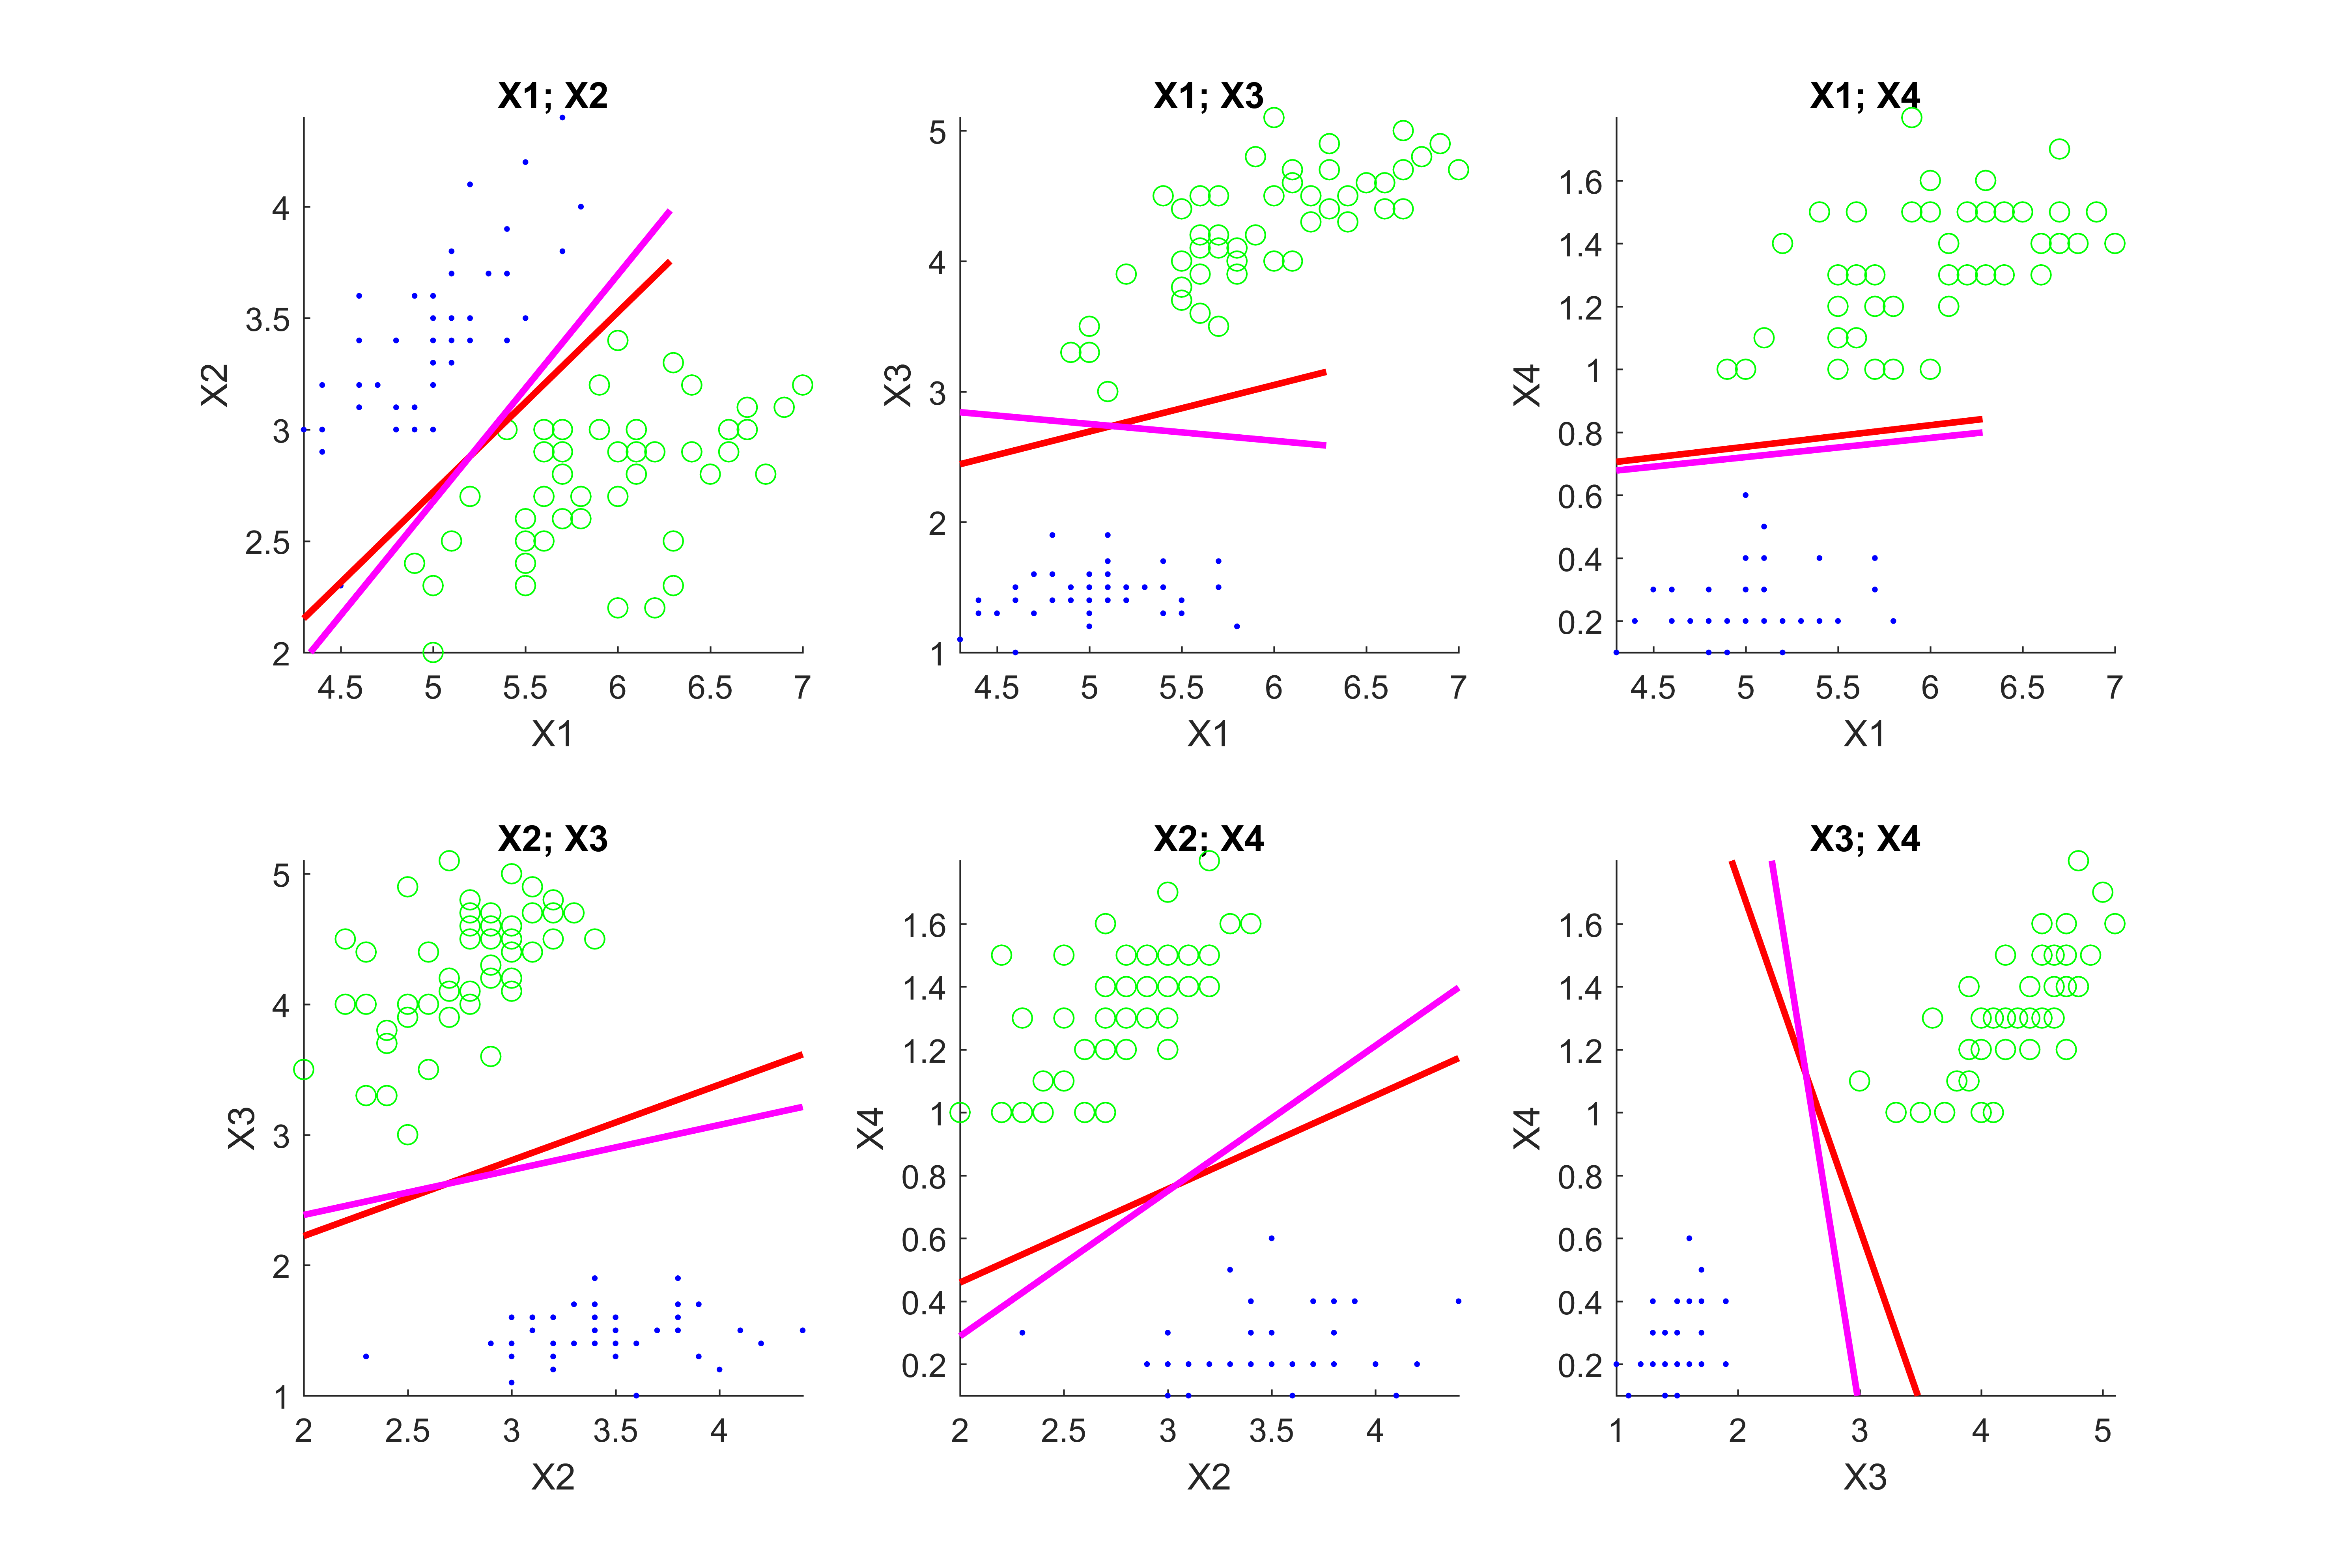
\includegraphics[width=6in]{p55.png}
		\caption{Problem 55: The naive Bayes and logistic classifiers are shown as red and magenta lines.}
	\end{center}
\end{figure}


The binary classification results are shown in Fig. 1 with the naive Bayes and logistic classifiers being the red and magenta lines respectively. 




\section*{Problem 57}

Please see the final section for the short report. 

\section*{Problem 58}

In this problem we explore the effects of gender and smoking on the  re-admission times of patients with cardiac arrhythmia. The data set \textit{arrhythmia.mat} has 100 observations and contains the time between the first and second admission to the hospital due to cardiac arrhythmia. Some of the data is right-censored with different censoring cutoff because contact to the patient might be lost at different time. The data is further labeled with the gender and smoker. A snippet of the data is shown in Table 1. 

\begin{table}[]
\centering
\begin{tabular}{|c|c|c|c|c|}
\hline
patient \# & Re-admission Time ($t_i$) & Censored & Gender & Smoker \\ \hline
1          & 5                 & 0        & 0      & 1      \\ \hline
2          & 3                 & 0        & 1      & 1      \\ \hline
3          & 19                & 1        & 1      & 0      \\ \hline
4          & 17                & 1        & 1      & 0      \\ \hline
\end{tabular}
\caption{\label{tab:tab1} A snippet of the \textit{arrhythmia.mat} data set.}
\end{table}

Let $t_i$ be the re-admission time observation of the $i$\textsuperscript{th} patient and $y_i$ be the real readmission time. For uncensored data, $t_i = y_i$ $\forall i = 1,2,\dots, n_{uc}$ while for censored data with cutoff $c_j$, $t_j = c_j$ $\forall j = 1,2,\dots, n_c$. We formulate the Poisson model with parameter $x$ to be estimated as the following. 
\begin{equation}
P(t_i = y_i|x) = \frac{e^{-x}x^{t_i}}{t_i!} \quad \forall i = 1,2,\dots, n_{uc}
\end{equation}
\begin{equation}
P(t_j = c_j|x) = \left(1 - \sum_{k=0}^{t_j}\frac{e^{-x}x^k}{k!} \right) \quad \forall j = 1,2,\dots, n_{c}
\end{equation}
The likelihood for the observed uncensored data $\{t_i\}_{i=1}^{n_{uc}}$ and censored data $\{t_j\}_{j=1}^{n_{c}}$ is 
\begin{equation}
P(\{t_i\}_{i=1}^{n_{uc}}; \{t_j\}_{j=1}^{n_{c}}|x) = \left(\prod_{i=1}^{n_{uc}}\frac{e^{-x}x^{t_i}}{t_i!} \right)\prod_{j=1}^{n_c}\left( 1 - \sum_{k=0}^{t_j}\frac{e^{-x}x^k}{k!} \right)
\end{equation}
We further assume the improper prior for the parameter $x$: $P(x) \sim \frac{1}{x}$ to evaluate the posterior distribution $P(x|\{t_i\}_{i=1}^{n_{uc}}; \{t_j\}_{j=1}^{n_{c}})$. We use Gibbs sampling to simulate a \textit{cloud} of the $x$ estimates and access the mean and variance of the estimate. For Gibbs sampling, we need to augment $\{y_j \}_{j=1}^{n_c}$ to the censored data and marginalize on $\{y_j \}_{j=1}^{n_c}$. We simulate the augmented data $\{y_j \}_{j=1}^{n_c}$ using the following probability distribution. 
\begin{equation}
P\left(y_j | \{t_i\}_{i=1}^{n_{uc}}, \{t_j\}_{j=1}^{n_{c}}, x \right) \propto \left(\frac{e^{-x}x^{y_j}}{y_j!} \right) I(y_j\geq t_j)
\end{equation}
Note that sampling from Eq. (22) is equivalent to sampling from a Poisson with mean $x$ and than adding a constant $t_j$. With all the augmented $\{y_j \}_{j=1}^{n_c}$, the posterior of $x$ is then
\begin{equation}
\begin{split}
P\left(x| \{t_i\}_{i=1}^{n_{uc}}, \{t_j\}_{j=1}^{n_{c}} \right) & = P\left( x| \{t_i\}_{i=1}^{n_{uc}}, \{y_j\}_{j=1}^{n_{c}} \right) \\
 & \propto \left(\prod_{i=1}^{n_{uc}}\frac{e^{-x}x^{t_i}}{t_i!} \right)\left(\prod_{j=1}^{n_{c}}\frac{e^{-x}x^{y_i}}{y_i!}  \right)\left( \frac{1}{x}\right)
\end{split}
\end{equation}
One way is to we simulate $\{y_j^{(k)} \}_{j=1}^{n_c}$ using Eq. (22) and $x^{(k)}$ using Eq. (23). The sequence $x^{(1)}, x^{(2)}, \dots, x^{(k)}$ converges to the posterior distribution $P(x|\{t_i\}_{i=1}^{n_{uc}}, \{t_j\}_{j=1}^{n_{c}})$. The other way (given the form of the posterior) is to use the MAP estimator derived as the following. 
\begin{equation}
L = \log \left[P\left( x| \{t_i\}_{i=1}^{n_{uc}}, \{y_j\}_{j=1}^{n_{c}} \right)\right]
\end{equation}
\begin{equation}
\frac{dL}{dx} = -(n_{uc}+n_c) + \frac{1}{x}\left(\sum_{i=1}^{n_{uc}}t_i + \sum_{j=1}^{n_c}y_j - 1 \right) = 0
\end{equation}
\begin{equation}
\hat{x}_{MAP} = \frac{\sum_{i=1}^{n_{uc}}t_i + \sum_{j=1}^{n_c}y_j - 1}{n_{uc}+n_c}
\end{equation}
As one side note, the prior $P(x) \propto \frac{1}{x}$ comes in as the $-1$ term. Given large number of observations, $n$, the effect of the prior dies with $\mathcal{O}(1/n)$.

\begin{figure}
	\begin{center}
		\includegraphics[width=6.5in]{p58.png}
		\caption{Problem 58: The histograms of $x$ estimate using Gibbs sampling to investigate the (left) gender effect (middle) smoking effect and (right) combined effect of the re-admission time for 100 patients with cardiac arrhythmia. The mean and standard deviation of $x$ estimate is reported in the legend where $n$ is the number of observations in the data set. } 
	\end{center}
\end{figure}

The distributions of $x$ estimate from Gibbs sampling is shown in Fig. 2 and we compare the gender, smoking effects as well as combined effects. From the data, the gender plays a much more important role in the re-admission time for the patients; male patients tend to have re-admission time of $2.37$ compare to $6.77$ of female patients. As expected smokers have shorter re-admission time. Therefore, using the Poisson likelihood and Gibbs sampling, we report that
\begin{equation}
x(\text{Female Nonsmoker}) > x(\text{Female Ssmoker}) > x(\text{Male Nonsmoker}) > x(\text{Male Smoker})
\end{equation}



\section*{Problem 59}

The nonlinear stochastic system is defined as the following. 
\begin{equation}
x_{k+1} = \sin(x_k) + x_k \quad w\sim N(0, \Sigma)
\end{equation}
Let the initial density of $x_0$ be $\pi_0(x)$ and we can write the transition probability from time $k$ to time $k+1$ as 
\begin{equation}
P(x_{k+1}|x_k) = N(\sin(x_k), \Sigma)
\end{equation}
By Chapman-Komogorov equation, the density of $x_{k+1}$ is $\pi_{k+1}(x_{k+1})$:
\begin{equation}
\pi_{k+1}(x_{k+1}) = \int P(x_{k+1}|x_k)\pi_k(x_k)dx_k
\end{equation}

Instead of doing the integration, we can simulate $x_{k+1}$'s using the composite method by knowing both $P(x_{k+1}|x_k)$ and $\pi_k(x_k)$. 
\begin{enumerate}
\item Generate $x_k^* \sim \pi_k(x_k)$ 
\item Generate $x_{k+1}^* \sim P(x_{k+1}|x_k^*)$
\end{enumerate}
The density of simulated $x_{k+1}^*$'s, $\hat{\pi}_{k+1}(x_{k+1})$ will converge to $\pi_{k+1}(x_{k+1})$. Using this simulated density, we can repeat the same procedure for $k+2$, $k+3$, etc. Note that we will have to generate $x_{k+1}^*$ from the empirical density $\hat{\pi}_{k+1}(x_{k+1})$ but the simulated $x_{k+1}^*$ is already determined. Therefore, to simulate this system for $k=1, 2, 3$, we use the following simplified procedure. 
\begin{enumerate}
\item Generate $x_0^* \sim \pi_0(x_0)$.
\item Generate $x_{1}^* \sim P(x_1|x_0^*) \to$ find density, mean and covariance, $k=1$. 
\item Generate $x_{2}^* \sim P(x_2|x_1^*) \to$ find density, mean and covariance, $k=2$.
\item Generate $x_{3}^* \sim P(x_3|x_2^*) \to$ find density, mean and covariance, $k=3$.
\end{enumerate}

\begin{figure}
	\begin{center}
		\includegraphics[width=6.5in]{p59.png}
		\caption{Problem 59: The densities of $x_0$, $x_1$, $x_2$ and $x_3$ from 2 simulations with $\Sigma_1$ and $\Sigma_2$.  } 
	\end{center}
\end{figure}

To run the simulation, suppose that $x$ is a normally distributed two-dimensional random vector with mean $\mu$ and covariance $I_2$, i.e. $x\sim N_2(\mu, I_2)$, where $\mu = (3, -2)'$ to demonstrate the non-linearity of the problem. We choose the two-dimensional example for the ease of visualization. We ran two simulations with different $\Sigma$'s:
\begin{equation}
\Sigma_1 = \begin{bmatrix}
1 & 1.5 \\
1.5 & 3
\end{bmatrix} \quad \Sigma_2 = \begin{bmatrix}
1 & -0.8 \\
-0.8 & 0.9
\end{bmatrix}
\end{equation}
and the simulated densities are shown in Fig. 3. We report the statistics as follows. 

For the first simulation, 
\begin{equation}
\bar{x_1} = \begin{bmatrix}
0.0923 \\
-0.5368
\end{bmatrix} \quad \bar{x_2} = \begin{bmatrix}
0.0527 \\
-0.1024
\end{bmatrix} \quad \bar{x_3} = \begin{bmatrix}
0.0281 \\
-0.0127
\end{bmatrix}
\end{equation}

\begin{equation}
\text{cov}(x_1) = \begin{bmatrix}
1.42 & 1.49 \\
1.49 & 3.21
\end{bmatrix} \quad \text{cov}(x_2) = \begin{bmatrix}
1.48 & 1.67 \\
1.67 & 3.49
\end{bmatrix} \quad \text{cov}(x_3) = \begin{bmatrix}
1.49 & 1.72 \\
1.72 & 3.50
\end{bmatrix}
\end{equation}

For the second simulation, 
\begin{equation}
\bar{x_1} = \begin{bmatrix}
0.1034 \\
-0.5611
\end{bmatrix} \quad \bar{x_2} = \begin{bmatrix}
0.0506 \\
-0.3136
\end{bmatrix} \quad \bar{x_3} = \begin{bmatrix}
0.0418 \\
-0.1974
\end{bmatrix}
\end{equation}

\begin{equation}
\text{cov}(x_1) = \begin{bmatrix}
1.46 & -0.82 \\
-0.82 & 1.13
\end{bmatrix} \quad \text{cov}(x_2) = \begin{bmatrix}
1.47 & -1.01 \\
-1.01 & 1.29
\end{bmatrix} \quad \text{cov}(x_3) = \begin{bmatrix}
1.50 & -1.10 \\
-1.10 & 1.36
\end{bmatrix}
\end{equation}




\section*{Problem 61}

Denote the state in the phase space as $z_k = (x_k,\dot{x}_k, y_k, \dot{y}_k)'$ and acceleration $r_{k+1} = (\ddot{x}_{k}, \ddot{y}_{k})'$, which will be deemed as a constant $r$. The state and the observation models are the following. 
\begin{equation}
z_{k+1} = Az_k+fr_{k+1}+w_k \quad w_k\sim(0, Q)\quad k=0,1,\dots
\end{equation}
\begin{equation}
y_k = Cz_k+v_k \quad v_k\sim N(0, R)
\end{equation}
where 
\begin{equation}
A = \begin{bmatrix}
1 & \Delta & 0 & 0\\
0& 1 & 0 & 0\\
0 & 0 & 1 & \Delta\\
0 & 0 & 0 & 1\\
\end{bmatrix}\quad f = \begin{bmatrix}
\Delta^2/2 & 0 \\
\Delta & 0 \\
0 & \Delta^2/2 \\
0 & \Delta\\
\end{bmatrix}\quad C = \begin{bmatrix}
1 & 0 & 0 & 0\\
0 & 0& 1 & 0
\end{bmatrix}
\end{equation}
and $\Delta$ is the sampling period. We will use Kalman Filter (KF) to estimate the state $x_k$ given observations $y_k$. We write the recursive KF equations as the following. 
\begin{equation}
\begin{split}
\hat{z}_{k+1|k} & = A\hat{z}_k + fr \\
y_{k+1|k} & = C\hat{z}_{k+1|k} \\
\Sigma_{k+1|k} & = A\Sigma_kA'+Q\\
S_{k+1} & = C\Sigma_{k+1|k}C'+R\\
\hat{z}_{k+1} & = \hat{z}_{k+1|k} + \Sigma_{k+1|k}C'S_{k+1}^{-1}(y_{k+1} - y_{k+1|k})\\
\Sigma_{k+1} & = \Sigma_{k+1|k}C'S_{k+1}^{-1}C\Sigma_{k+1|k}
\end{split}
\end{equation}


\begin{figure}
\centering
\begin{subfigure}[]{}
   \includegraphics[width=6.5in]{p61_1.png}
\end{subfigure}

\begin{subfigure}[]{}
   \includegraphics[width=6.5in]{p61_2.png}
\end{subfigure}

\begin{subfigure}[]{}
   \includegraphics[width=6.5in]{p61_3.png}
\end{subfigure}

\caption{Problem 61: Simulated positions (black traces in the left 2 panels), velocities traces (blue and red in the right panel) and noisy observations (blue in the left panel) using Eq. (36) and (37). The position traces of KF estimate are shown as red dashed lines in the middle panel while the KF estimate of velocities are shown as cyan and magenta in the right panel. We use three different noise levels: $\sigma^2R$ with (a) $\sigma^2=1$, (b) $\sigma^2=5$ and (c) $\sigma^2=10$.}
\end{figure}


We simulate the observations using three different noise levels $\sigma^2R$ where $\sigma^2R$ with $\sigma^2=1,5,10$. The results are shown in Fig. 4. The KF filter works very well even in the most noisy case; the KF estimates still recapitulate the positions of the target. It is interesting to note that the KF estimates for the velocities are not as good as the positions because in the observation matrix $C$, we do not observe the velocities. However, the KF estimates of the velocities seem to be insensitive to the observation noise because the velocities are inferred instead of being corrupted measurements. This problem demonstrate decent performance of Kalman Filter even though the observation is highly noisy. 






\section*{Problem 62}

Suppose we have the transition matrix $p\in\mathbb{R}^{3\times 3}$ for the Markov Chain $x_k$ in state space $\{0, 10, 20\}$ and let $\pi_k(i) = P(x_k=i|y_{1:k})$. Now the observation of the Markov Chain is noisy: 
\begin{equation}
y_{k} = x_k + w \quad w\sim N(0, \sigma^2)
\end{equation}

\subsection*{(a)}

The probability of observation $y_k$ given state at $x_k$ is 
\begin{equation}
P(y_k|x_k) = N(x_k, \sigma^2)
\end{equation}
Note that $x_k$ is discrete from a 3-state Markov Chain while $y_k$ is a continuous observation. We apply the Hidden Markov Model (HMM) Filter using the following state estimate $\pi_{k+1}$ given observation $y_{1:k+1}$: 
\begin{equation}
\pi_{k+1} = \frac{B_{y_{k+1}}P'\pi_k}{\mathbf{1}'B_{y_{k+1}}P'\pi_k} \quad B_{y_k} = \begin{bmatrix}
P(y_k|x_k=0) & 0 & 0 \\
0 & P(y_k|x_k=10) & 0 \\
0 & 0 & P(y_k|x_k=20)
\end{bmatrix}
\end{equation}
Let $S = (0, 10, 20)'$ be the state vector. The optimal estimate from the HMM filter is
\begin{equation}
\hat{x}_{k+1} = S'\pi_{k+1}
\end{equation}

\begin{figure}
	\begin{center}
		\includegraphics[width=6.5in]{p62.png}
		\caption{Problem 62(a): The simulated noisy measurements $y_k$ (blue) of Markov Chain states $x_k$ (black) using $\sigma^2=1$, $\sigma^2=2$ and $\sigma^2=5$. The red dashed traces represents the estimates from HMM filter. The magenta dots indicate the time $k$ when the HMM estimate $\hat{x}_k$ does not agree with the true state $x_k$. } 
	\end{center}
\end{figure}

The traces of the simulated Markov Chain $x_k$ and the noisy observations $y_k$ with $\sigma^2 = 1,2,5$ are shown as blue and black respectively in Fig. 5. The trace of estimate from HMM filter, $\hat{x}_k$ is shown in the red dashed line. In general, HMM filter performs very well in this case, where for different observation noises, the most of the estimates recapitulate the hidden Markov Chain. We indicate the disagreement using the magenta dots in Fig. 5 and with increasing $\sigma^2$, the error occurs more frequently due to the high noisy once in a while. We report the error rate $r$ for three different cases as the following. 
\begin{equation}
\begin{split}
\sigma^2 = 1 \quad & r = 0.00\% \\
\sigma^2 = 2 \quad & r = 0.20\% \\
\sigma^2 = 5 \quad & r = 5.50\% \\
\end{split}
\end{equation}
The good performance is also due to the fact that the differences between the Markov states are big enough that the noises do not corrupt the signal significantly even for the case where $\sigma^2=5$. 


\subsection*{(b)}

\begin{figure}
	\begin{center}
		\includegraphics[width=6.5in]{p62b.png}
		\caption{Problem 62(b): The simulated noisy measurements $y_k$ (blue) of Markov Chain states $x_k$ (black) using $\sigma^2=1$, $\sigma^2=2$ and $\sigma^2=5$. The red dashed traces represents the estimates from fixed interval smoothed estimate (FISE) using the Viterbi algorithm. The magenta dots indicate the time $k$ when the FISE estimate $\hat{x}_k$ does not agree with the true state $x_k$. } 
	\end{center}
\end{figure}

We further use a fixed interval smoothed estimate (FISE) for the Markov state $x_k$ using the Viterbi algorithm. In the Viterbi algorithm, we have to maximize the likelihood $P(y_{1:k}, x_{1:k})$ and since the Markov state $x_k$ is equally spaced with the same observation noise variance, the maximum-likelihood estimate for state at time $k$ given observation $y_k$ is essentially rounding the observation to the closest state. The red dashed lines in Fig. 6 demonstrate the traces FISE from the same observations $y_{1:1000}$. Using the same plotting scheme, we label the disagreement between FISE and real state by the magenta dots and report the error rates as the following. 
\begin{equation}
\begin{split}
\sigma^2 = 1 \quad & r = 0.00\% \\
\sigma^2 = 2 \quad & r = 0.10\% \\
\sigma^2 = 5 \quad & r = 1.30\% \\
\end{split}
\end{equation}


\section*{Attachments}
\textit{to be updated}



\end{document}
